\documentclass[xetex,mathserif,serif]{beamer}
\usepackage{polyglossia}
\setdefaultlanguage[babelshorthands=true]{russian}
\usepackage{minted}
\usepackage{tabu}

\useoutertheme{infolines}

\usepackage{fontspec}
\setmainfont{FreeSans}
\newfontfamily{\russianfonttt}{FreeSans}

\definecolor{links}{HTML}{2A1B81}
\hypersetup{colorlinks,linkcolor=,urlcolor=links}

\tabulinesep=0.8mm

\title{Аннотации, процессоры аннотаций, Lombok}
\author[Юрий Литвинов]{Юрий Литвинов \newline \textcolor{gray}{\small\texttt{yurii.litvinov@gmail.com}}}

\date{27.04.2018г}

\begin{document}
	
	\frame{\titlepage}

	\section{Аннотации}

	\begin{frame}
		\frametitle{Аннотации}
		\begin{itemize}
			\item Нужны для добавления метаданных в классы
			\begin{itemize}
				\item Могут потом использоваться во время компиляции или во время выполнения
				\item Активно используются самим компилятором (\mintinline{java}|@Override|, \mintinline{java}|@SuppressWarnings|)
			\end{itemize}
			\item Могут использоваться для генерации кода во время компиляции (например, Lombok)
			\item Полезны во время выполнения вместе с рефлексией (например, JUnit)
		\end{itemize}
	\end{frame}

	\begin{frame}[fragile]
		\frametitle{Объявление своей аннотации}
		\begin{minted}{java}
@Target(ElementType.TYPE)
@Retention(RetentionPolicy.RUNTIME)
public @interface Mammal {
    String sound();
    int color();
}
		\end{minted}
	\end{frame}

	\begin{frame}[fragile]
		\frametitle{Использование}
		\begin{minted}{java}
@Mammal(color = 0xFFA844, sound = "uuuu")
class Giraffe {
}
		\end{minted}
	\end{frame}

	\begin{frame}[fragile]
		\frametitle{Работа с аннотациями в рантайме}
		\begin{minted}{java}
@PermissionRequired(User.Permission.USER_MANAGEMENT)
class UserDeleteAction {
    public void invoke(User user) { /* */ }
}

User user = ...;
Class<?> actionClass = ...;
PermissionRequired permissionRequired =
        actionClass.getAnnotation(PermissionRequired.class);
if (permissionRequired != null)
    if (user != null && user.getPermissions().contains(
        permissionRequired.value())) {
            // выполнить действие
        }
    }
}
		\end{minted}
	\end{frame}
	
	\section{Процессоры аннотаций}

	\begin{frame}
		\frametitle{Процессоры аннотаций}
		\begin{itemize}
			\item Обрабатывают аннотации во время компиляции
			\begin{itemize}
				\item Можно понимать как плагины к компилятору
			\end{itemize}
			\item Генерируют код
			\begin{itemize}
				\item Который потом подаётся на вход компилятору
			\end{itemize}
			\item Появились в Java 6
			\item Используются многими библиотеками
		\end{itemize}
	\end{frame}

	\begin{frame}[fragile]
		\frametitle{API}
		\begin{small}
			\begin{minted}{java}
public class MyProcessor extends AbstractProcessor {

    @Override
    public synchronized void init(ProcessingEnvironment env) { }

    @Override
    public boolean process(
        Set<? extends TypeElement> annotations, 
        RoundEnvironment env) { }

    @Override
    public Set<String> getSupportedAnnotationTypes() { }

    @Override
    public SourceVersion getSupportedSourceVersion() { }
}
			\end{minted}
		\end{small}
	\end{frame}

	\begin{frame}[fragile]
		\frametitle{API, с Java 7}
		\begin{small}
			\begin{minted}{java}
@SupportedSourceVersion(SourceVersion.latestSupported())
@SupportedAnnotationTypes({...})
public class MyProcessor extends AbstractProcessor {

    @Override
    public synchronized void init(
        ProcessingEnvironment env) { }

    @Override
    public boolean process(
        Set<? extends TypeElement> annoations, 
        RoundEnvironment env) { }
}
			\end{minted}
		\end{small}
	\end{frame}

	\begin{frame}[fragile]
		\frametitle{Регистрация процессора}
		Надо собрать специальный jar-файл
		\begin{minted}{text}
MyProcessor.jar
    - com
        - example
            - MyProcessor.class

    - META-INF
        - services
            - javax.annotation.processing.Processor
		\end{minted}
		javax.annotation.processing.Processor содержит полностью квалифицированные имена классов-процессоров через перевод строки
	\end{frame}

	\begin{frame}[fragile]
		\frametitle{Компиляция кода с процессором}
		Добавить процессор в classpath (на самом деле, в -processorpath у javac)
		\vspace{1cm}
		\begin{minted}{text}
>javac -cp com.example.annotations.jar;
     com.example.annotations.processors.jar
     MyCode.java
		\end{minted}
	\end{frame}

	\section{Пример: фабрика}

		\begin{frame}[fragile]
		\frametitle{Пример: фабрика}
		\begin{footnotesize}
			\begin{minted}{java}
public interface Meal {
  public float getPrice();
}
public class MargheritaPizza implements Meal {
  @Override public float getPrice() {
    return 6.0f;
  }
}
public class CalzonePizza implements Meal {
  @Override public float getPrice() {
    return 8.5f;
  }
}
public class Tiramisu implements Meal {
  @Override public float getPrice() {
    return 4.5f;
  }
}
			\end{minted}
		\end{footnotesize}
	\end{frame}

	\begin{frame}[fragile]
		\frametitle{Основной класс}
		\begin{small}
			\begin{minted}{java}
public class PizzaStore {

  private MealFactory factory = new MealFactory();

  public Meal order(String mealName) {
    return factory.create(mealName);
  }

  public static void main(String[] args) throws IOException {
    PizzaStore pizzaStore = new PizzaStore();
    Meal meal = pizzaStore.order(readConsole());
    System.out.println("Bill: " + meal.getPrice());
  }
}
			\end{minted}
		\end{small}
	\end{frame}

	\begin{frame}[fragile]
		\frametitle{Фабрика}
		\begin{small}
			\begin{minted}{java}
public class MealFactory {

  public Meal create(String id) {
    if (id == null) {
      throw new IllegalArgumentException("id is null!");
    } else if ("Calzone".equals(id)) {
      return new CalzonePizza();
    } else if ("Tiramisu".equals(id)) {
      return new Tiramisu();
    } else if ("Margherita".equals(id)) {
      return new MargheritaPizza();
    }

    throw new IllegalArgumentException("Unknown id = " + id);
  }
}
			\end{minted}
		\end{small}
	\end{frame}

	\begin{frame}[fragile]
		\frametitle{Аннотация @Factory}
		\begin{small}
			\begin{minted}{java}
@Target(ElementType.TYPE) 
@Retention(RetentionPolicy.CLASS)
public @interface Factory {

  /** The name of the factory */
  Class type();

  /** The identifier for determining which item should be instantiated */
  String id();
}
			\end{minted}
		\end{small}
	\end{frame}

	\begin{frame}[fragile]
		\frametitle{Пиццы}
		\begin{small}
			\begin{minted}{java}
@Factory(id = "Margherita", type = Meal.class)
public class MargheritaPizza implements Meal {
  @Override public float getPrice() {
    return 6f;
  }
}

@Factory(id = "Calzone", type = Meal.class)
public class CalzonePizza implements Meal {
  @Override public float getPrice() {
    return 8.5f;
  }
}
			\end{minted}
		\end{small}
	\end{frame}

	\begin{frame}[fragile]
		\frametitle{Самое интересное: процессор}
		\begin{scriptsize}
			\begin{minted}{java}
@AutoService(Processor.class)
public class FactoryProcessor extends AbstractProcessor {
  private Types typeUtils;
  private Elements elementUtils;
  private Filer filer;
  private Messager messager;
  private Map<String, FactoryGroupedClasses> factoryClasses 
      = new LinkedHashMap<String, FactoryGroupedClasses>();
  @Override
  public synchronized void init(ProcessingEnvironment processingEnv) {
    super.init(processingEnv);
    typeUtils = processingEnv.getTypeUtils();
    elementUtils = processingEnv.getElementUtils();
    filer = processingEnv.getFiler();
    messager = processingEnv.getMessager();
  }
  @Override
  public Set<String> getSupportedAnnotationTypes() {
    Set<String> annotations = new LinkedHashSet<String>();
    annotations.add(Factory.class.getCanonicalName());
    return annotations;
  }
  ...
}
			\end{minted}
		\end{scriptsize}
	\end{frame}

	\begin{frame}[fragile]
		\frametitle{Элементы}
		\begin{small}
			\begin{minted}{java}
package com.example;    // PackageElement

public class Foo {      // TypeElement

    private int a;      // VariableElement
    private Foo other;  // VariableElement

    public Foo () {}    // ExecuteableElement

    public void setA (  // ExecuteableElement
        int newA        // VariableElement
        ) {}
}
			\end{minted}
		\end{small}
	\end{frame}

	\begin{frame}[fragile]
		\frametitle{Пример работы с элементами}
		\begin{minted}{java}
TypeElement fooClass = ...;
for (Element e : fooClass.getEnclosedElements()) {
    Element parent = e.getEnclosingElement();
}
		\end{minted}
	\end{frame}

	\begin{frame}[fragile]
		\frametitle{Вернёмся к процессору}
		\begin{minted}{java}
@AutoService(Processor.class)
public class FactoryProcessor extends AbstractProcessor {
  ...
  @Override
  public boolean process(
      Set<? extends TypeElement> annotations, 
      RoundEnvironment roundEnv) {
    // Iterate over all @Factory annotated elements
    for (Element annotatedElement 
        : roundEnv.getElementsAnnotatedWith(Factory.class)) {
      ...
    }
  }
 ...
}
		\end{minted}
	\end{frame}

	\begin{frame}[fragile]
		\frametitle{FactoryAnnotatedClass}
		\begin{footnotesize}
			\begin{minted}{java}
public class FactoryAnnotatedClass {
    private TypeElement annotatedClassElement; 
    private String qualifiedSuperClassName;
    private String simpleTypeName; 
    private String id;
    public FactoryAnnotatedClass(TypeElement classElement) 
            throws IllegalArgumentException {
    this.annotatedClassElement = classElement;
    Factory annotation = classElement.getAnnotation(Factory.class);
    id = annotation.id(); 
    if (StringUtils.isEmpty(id)) {
        throw new IllegalArgumentException(
                String.format("id() in @%s for class %s is null or empty! that's not allowed",
                Factory.class.getSimpleName(), classElement.getQualifiedName().toString()));
    }
    ...
			\end{minted}
		\end{footnotesize}
	\end{frame}

	\begin{frame}[fragile]
		\frametitle{FactoryAnnotatedClass (2)}
		\begin{footnotesize}
			\begin{minted}{java}
public class FactoryAnnotatedClass {
    public FactoryAnnotatedClass(TypeElement classElement) 
            throws IllegalArgumentException {
    ...
    try {
        Class<?> clazz = annotation.type();
        qualifiedSuperClassName = clazz.getCanonicalName();
        simpleTypeName = clazz.getSimpleName();
    } catch (MirroredTypeException mte) {
        DeclaredType classTypeMirror = (DeclaredType) mte.getTypeMirror();
        TypeElement classTypeElement = (TypeElement) classTypeMirror.asElement();
        qualifiedSuperClassName = classTypeElement.getQualifiedName().toString();
        simpleTypeName = classTypeElement.getSimpleName().toString();
    }
}
			\end{minted}
		\end{footnotesize}
	\end{frame}

	\begin{frame}[fragile]
		\frametitle{FactoryGroupedClasses}
		\begin{footnotesize}
			\begin{minted}{java}
public class FactoryGroupedClasses {
    private String qualifiedClassName;
    private Map<String, FactoryAnnotatedClass> itemsMap =
            new LinkedHashMap<String, FactoryAnnotatedClass>();
    public FactoryGroupedClasses(String qualifiedClassName) {
        this.qualifiedClassName = qualifiedClassName;
    }
    public void add(FactoryAnnotatedClass toInsert) throws IdAlreadyUsedException {
        FactoryAnnotatedClass existing = itemsMap.get(toInsert.getId());
        if (existing != null) {
            throw new IdAlreadyUsedException(existing);
        }
        itemsMap.put(toInsert.getId(), toInsert);
    }
    public void generateCode(Elements elementUtils, Filer filer) throws IOException {
        ...
    }
}
			\end{minted}
		\end{footnotesize}
	\end{frame}

	\begin{frame}[fragile]
		\frametitle{Вернёмся к процессору ещё раз}
		\begin{footnotesize}
			\begin{minted}{java}
public class FactoryProcessor extends AbstractProcessor {
    @Override
    public boolean process(Set<? extends TypeElement> annotations, 
            RoundEnvironment roundEnv) {
        for (Element annotatedElement 
                : roundEnv.getElementsAnnotatedWith(Factory.class)) {
            ...
            TypeElement typeElement = (TypeElement) annotatedElement;
            try {
                FactoryAnnotatedClass annotatedClass =
                        new FactoryAnnotatedClass(typeElement); 
                if (!isValidClass(annotatedClass)) {
                    return true; 
                }
            } catch (IllegalArgumentException e) {
                error(typeElement, e.getMessage());
                return true;
            }
            ...
        }
			\end{minted}
		\end{footnotesize}
	\end{frame}

	\begin{frame}[fragile]
		\frametitle{Продолжим}
		\begin{footnotesize}
			\begin{minted}{java}
try {
    FactoryAnnotatedClass annotatedClass = new FactoryAnnotatedClass(typeElement);
    if (!isValidClass(annotatedClass)) {
        return true; // Error message printed, exit processing
    }
    // Everything is fine, so try to add
    FactoryGroupedClasses factoryClass =
            factoryClasses.get(annotatedClass.getQualifiedFactoryGroupName());
    if (factoryClass == null) {
        String qualifiedGroupName = annotatedClass.getQualifiedFactoryGroupName();
        factoryClass = new FactoryGroupedClasses(qualifiedGroupName);
        factoryClasses.put(qualifiedGroupName, factoryClass);
    }
    factoryClass.add(annotatedClass);
} catch (IllegalArgumentException e) {
    // @Factory.id() is empty --> printing error message
} catch (IdAlreadyUsedException e) {
    // Already existing
}
			\end{minted}
		\end{footnotesize}
	\end{frame}

	\begin{frame}[fragile]
		\frametitle{И генерация кода}
		\begin{footnotesize}
			\begin{minted}{java}
@Override
public boolean process(Set<? extends TypeElement> annotations, 
        RoundEnvironment roundEnv) {
    ...
    try {
        for (FactoryGroupedClasses factoryClass : factoryClasses.values()) {
            factoryClass.generateCode(elementUtils, filer);
        }
    } catch (IOException e) {
        error(null, e.getMessage());
    }
    return true;
}
			\end{minted}
		\end{footnotesize}
	\end{frame}

	\begin{frame}[fragile]
		\frametitle{Собственно, генерация}
		\begin{footnotesize}
			\begin{minted}{java}
public class FactoryGroupedClasses {
    private static final String SUFFIX = "Factory";
    private String qualifiedClassName;
    private Map<String, FactoryAnnotatedClass> itemsMap =
            new LinkedHashMap<String, FactoryAnnotatedClass>();
    ...
    public void generateCode(Elements elementUtils, Filer filer) throws IOException {
        TypeElement superClassName = elementUtils.getTypeElement(qualifiedClassName);
        String factoryClassName = superClassName.getSimpleName() + SUFFIX;
        JavaFileObject jfo = filer.createSourceFile(qualifiedClassName + SUFFIX);
        Writer writer = jfo.openWriter();
        JavaWriter jw = new JavaWriter(writer);
        PackageElement pkg = elementUtils.getPackageOf(superClassName);
        if (!pkg.isUnnamed()) {
            jw.emitPackage(pkg.getQualifiedName().toString());
            jw.emitEmptyLine();
        } else {
            jw.emitPackage("");
        }
			\end{minted}
		\end{footnotesize}
	\end{frame}

	\begin{frame}[fragile]
		\frametitle{Собственно, генерация (2)}
		\begin{footnotesize}
			\begin{minted}{java}
        jw.beginType(factoryClassName, "class", EnumSet.of(Modifier.PUBLIC));
        jw.emitEmptyLine();
        jw.beginMethod(qualifiedClassName, "create", 
                EnumSet.of(Modifier.PUBLIC), "String", "id");
        jw.beginControlFlow("if (id == null)");
        jw.emitStatement("throw new IllegalArgumentException(\"id is null!\")");
        jw.endControlFlow();
        for (FactoryAnnotatedClass item : itemsMap.values()) {
            jw.beginControlFlow("if (\"%s\".equals(id))", item.getId());
            jw.emitStatement("return new %s()", 
                    item.getTypeElement().getQualifiedName().toString());
            jw.endControlFlow();
            jw.emitEmptyLine();
        }
        jw.emitStatement("throw new IllegalArgumentException(\"Unknown id = \" + id)");
        jw.endMethod();
        jw.endType();
        jw.close();
    }
}
			\end{minted}
		\end{footnotesize}
	\end{frame}

	\begin{frame}
		\frametitle{Полезные ссылки}
		\begin{itemize}
			\item \url{http://hannesdorfmann.com/annotation-processing/annotationprocessing101}
			\item \url{https://deors.wordpress.com/2011/10/08/annotation-processors/}
		\end{itemize}
	\end{frame}

	\section{Lombok}

	\begin{frame}
		\frametitle{Lombok}
		\begin{itemize}
			\item Очень известная библиотека аннотаций и процессоров, делающая программирование на Java несколько менее неудобным
			\item \url{https://projectlombok.org/}
			\item Генерирует boilerplate-код
			\begin{itemize}
				\item Геттеры и сеттеры
				\item Конструкторы
				\item Метод toString
				\item Методы equals и hashCode
				\item Всё это сразу
				\item Безопасный synchronized
				\item Строитель (Builder)
			\end{itemize}
		\end{itemize}
	\end{frame}

	\begin{frame}
		\frametitle{Что надо сделать}
		\begin{enumerate}
			\item Подключить артефакт org.projectlombok:lombok как compileOnly-зависимость
			\item Включить процессоры аннотаций в IDEA
			\begin{itemize}
				\item File -> Settings... -> Build, Execution, Deployment -> Compiler -> Annotation Processors
			\end{itemize}
		\end{enumerate}
		\begin{center}
			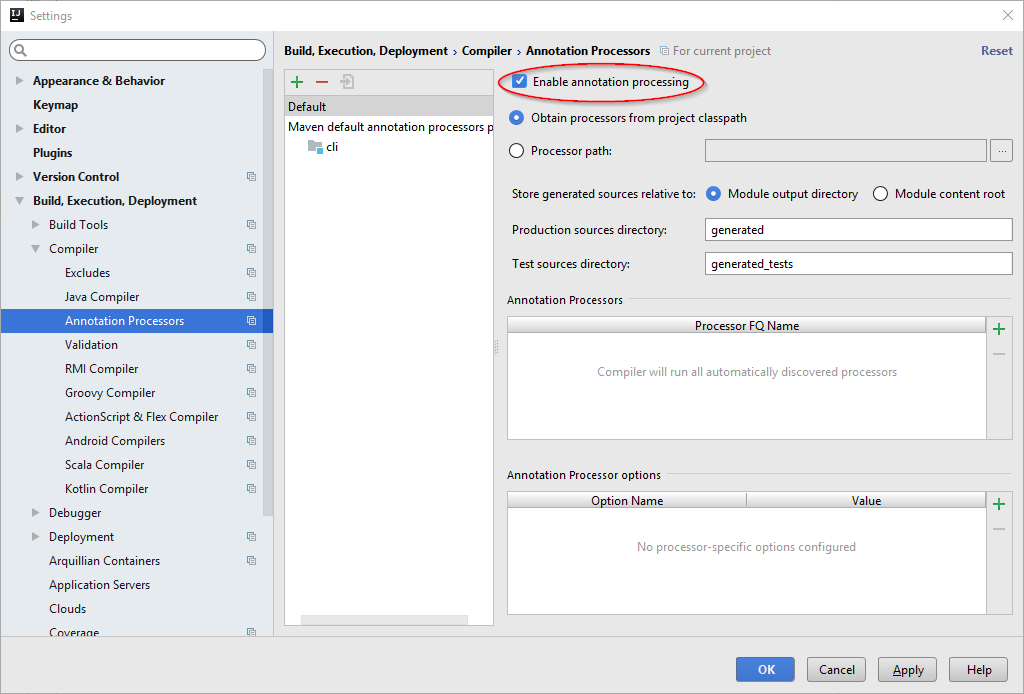
\includegraphics[width=0.6\textwidth]{annotationProcessors.png}
		\end{center}
	\end{frame}

	\begin{frame}[fragile]
		\frametitle{Геттеры и сеттеры}
		\begin{footnotesize}
			\begin{minted}{java}
@Getter @Setter private boolean employed = true;
@Setter(AccessLevel.PROTECTED) private String name;
		\end{minted}
		Эквивалентный код:
		\begin{minted}{java}
private boolean employed = true;
private String name;

public boolean isEmployed() {
    return employed;
}

public void setEmployed(final boolean employed) {
    this.employed = employed;
}

protected void setName(final String name) {
    this.name = name;
}
			\end{minted}
		\end{footnotesize}
	\end{frame}

	\begin{frame}[fragile]
		\frametitle{@ToString}
		\begin{footnotesize}
			\begin{minted}{java}
@ToString(callSuper=true,exclude="someExcludedField")
public class Foo extends Bar {
    private boolean someBoolean = true;
    private String someStringField;
    private float someExcludedField;
}
		\end{minted}
		Эквивалентный код:
		\begin{minted}{java}
public class Foo extends Bar {
    private boolean someBoolean = true;
    private String someStringField;
    private float someExcludedField;
    
    @java.lang.Override
    public java.lang.String toString() {
        return "Foo(super=" + super.toString() +
            ", someBoolean=" + someBoolean +
            ", someStringField=" + someStringField + ")";
    }
}
			\end{minted}
		\end{footnotesize}
	\end{frame}

	\begin{frame}[fragile]
		\frametitle{@EqualsAndHashCode}
		\begin{footnotesize}
			\begin{minted}{java}
@EqualsAndHashCode(callSuper=true, exclude={ "address", "city", "state", "zip" })
public class Person extends SentientBeing {
    enum Gender { Male, Female }

    @NonNull private String name;
    @NonNull private Gender gender;
    
    private String ssn;
    private String address;
    private String city;
    private String state;
    private String zip;
}
			\end{minted}
		\end{footnotesize}
	\end{frame}

	\begin{frame}[fragile]
		\frametitle{@Data}
		\begin{minted}{java}
@Data(staticConstructor="of")
public class Company {
    private final Person founder;
    private String name;
    private List<Person> employees;
}
		\end{minted}
	\end{frame}

	\begin{frame}[fragile]
		\frametitle{@Synchronized}
		\begin{small}
			\begin{minted}{java}
private DateFormat format = new SimpleDateFormat("MM-dd-YYYY");

@Synchronized
public String synchronizedFormat(Date date) {
    return format.format(date);
}
		\end{minted}
		Эквивалентный код:
		\begin{minted}{java}
private final java.lang.Object $lock = new java.lang.Object[0];
private DateFormat format = new SimpleDateFormat("MM-dd-YYYY");

public String synchronizedFormat(Date date) {
    synchronized ($lock) {  
        return format.format(date);
    }
}
			\end{minted}
		\end{small}
	\end{frame}

	\begin{frame}[fragile]
		\frametitle{@Builder}
		\begin{minted}{java}
 @Builder
 class Example {
        private int foo;
        private final String bar;
 }
		\end{minted}
	\end{frame}

	\begin{frame}[fragile]
		\frametitle{@Builder, эквивалентный код}
		\begin{tiny}
			\begin{minted}{java}
 class Example<T> {
        private T foo;
        private final String bar;
        
        private Example(T foo, String bar) {
                this.foo = foo;
                this.bar = bar;
        }        
        public static <T> ExampleBuilder<T> builder() {
                return new ExampleBuilder<T>();
        }        
        public static class ExampleBuilder<T> {
                private T foo;
                private String bar;
                private ExampleBuilder() {}
                public ExampleBuilder foo(T foo) {
                        this.foo = foo;
                        return this;
                }                
                public ExampleBuilder bar(String bar) {
                        this.bar = bar;
                        return this;
                }                
                @java.lang.Override public String toString() {
                        return "ExampleBuilder(foo = " + foo + ", bar = " + bar + ")";
                }                
                public Example build() {
                        return new Example(foo, bar);
                }
        }
 } 
			\end{minted}
		\end{tiny}
	\end{frame}

	\begin{frame}[fragile]
		\frametitle{@val}
		\begin{minted}{java}
val x = 10.0;
val y = new ArrayList<String>();
		\end{minted}
		\begin{itemize}
			\item Требует \mintinline{java}|import lombok.val;|
			\item Выводит тип из выражения инициализации
			\item Делает переменную \mintinline{java}|final|
		\end{itemize}
	\end{frame}

	\begin{frame}
		\frametitle{Домашка, MyJUnit}
		\framesubtitle{Последняя!}
		Реализовать command-line приложение, принимающее на вход путь и выполняющее запуск тестов, расположенных по этому пути
		\begin{itemize}
			\item Тестом считается метод, помеченный аннотацией Test
			\begin{itemize}
				\item У аннотации может быть два аргумента --- expected для исключения, ignore --- для отмены запуска и указания причины
			\end{itemize}
			\item Перед и после запуска каждого теста в классе должны запускаться методы, помеченные аннотациями Before и After
			\item Перед и после запуска тестов в классе должны запускаться методы, помеченные аннотациями BeforeClass и AfterClass
		\end{itemize}
	\end{frame}

	\begin{frame}
		\frametitle{Домашка, MyJUnit (2)}
		Приложение должно выводить в стандартный поток вывода отчет:
		\begin{itemize}
			\item о результате и времени выполнения прошедших и упавших тестов
			\item о причине отключенных тестов
		\end{itemize}
		Дедлайн: \textbf{18.05.2018, 10:00}
	\end{frame}

\end{document}
